% Generated by Sphinx.
\def\sphinxdocclass{report}
\documentclass[letterpaper,10pt,openany, oneside]{sphinxmanual}
\usepackage[utf8]{inputenc}
\DeclareUnicodeCharacter{00A0}{\nobreakspace}
\usepackage{cmap}
\usepackage[T1]{fontenc}
\usepackage[english]{babel}
\usepackage{times}
\usepackage[Bjarne]{fncychap}
\usepackage{longtable}
\usepackage{sphinx}
\usepackage{multirow}



\title{teakwood Documentation}
\date{October 13, 2014}
\release{1.0}
\author{Teakwood Group}
\newcommand{\sphinxlogo}{}
\renewcommand{\releasename}{Release}
\makeindex

\makeatletter
\def\PYG@reset{\let\PYG@it=\relax \let\PYG@bf=\relax%
    \let\PYG@ul=\relax \let\PYG@tc=\relax%
    \let\PYG@bc=\relax \let\PYG@ff=\relax}
\def\PYG@tok#1{\csname PYG@tok@#1\endcsname}
\def\PYG@toks#1+{\ifx\relax#1\empty\else%
    \PYG@tok{#1}\expandafter\PYG@toks\fi}
\def\PYG@do#1{\PYG@bc{\PYG@tc{\PYG@ul{%
    \PYG@it{\PYG@bf{\PYG@ff{#1}}}}}}}
\def\PYG#1#2{\PYG@reset\PYG@toks#1+\relax+\PYG@do{#2}}

\expandafter\def\csname PYG@tok@gd\endcsname{\def\PYG@tc##1{\textcolor[rgb]{0.63,0.00,0.00}{##1}}}
\expandafter\def\csname PYG@tok@gu\endcsname{\let\PYG@bf=\textbf\def\PYG@tc##1{\textcolor[rgb]{0.50,0.00,0.50}{##1}}}
\expandafter\def\csname PYG@tok@gt\endcsname{\def\PYG@tc##1{\textcolor[rgb]{0.00,0.27,0.87}{##1}}}
\expandafter\def\csname PYG@tok@gs\endcsname{\let\PYG@bf=\textbf}
\expandafter\def\csname PYG@tok@gr\endcsname{\def\PYG@tc##1{\textcolor[rgb]{1.00,0.00,0.00}{##1}}}
\expandafter\def\csname PYG@tok@cm\endcsname{\let\PYG@it=\textit\def\PYG@tc##1{\textcolor[rgb]{0.25,0.50,0.56}{##1}}}
\expandafter\def\csname PYG@tok@vg\endcsname{\def\PYG@tc##1{\textcolor[rgb]{0.73,0.38,0.84}{##1}}}
\expandafter\def\csname PYG@tok@m\endcsname{\def\PYG@tc##1{\textcolor[rgb]{0.13,0.50,0.31}{##1}}}
\expandafter\def\csname PYG@tok@mh\endcsname{\def\PYG@tc##1{\textcolor[rgb]{0.13,0.50,0.31}{##1}}}
\expandafter\def\csname PYG@tok@cs\endcsname{\def\PYG@tc##1{\textcolor[rgb]{0.25,0.50,0.56}{##1}}\def\PYG@bc##1{\setlength{\fboxsep}{0pt}\colorbox[rgb]{1.00,0.94,0.94}{\strut ##1}}}
\expandafter\def\csname PYG@tok@ge\endcsname{\let\PYG@it=\textit}
\expandafter\def\csname PYG@tok@vc\endcsname{\def\PYG@tc##1{\textcolor[rgb]{0.73,0.38,0.84}{##1}}}
\expandafter\def\csname PYG@tok@il\endcsname{\def\PYG@tc##1{\textcolor[rgb]{0.13,0.50,0.31}{##1}}}
\expandafter\def\csname PYG@tok@go\endcsname{\def\PYG@tc##1{\textcolor[rgb]{0.20,0.20,0.20}{##1}}}
\expandafter\def\csname PYG@tok@cp\endcsname{\def\PYG@tc##1{\textcolor[rgb]{0.00,0.44,0.13}{##1}}}
\expandafter\def\csname PYG@tok@gi\endcsname{\def\PYG@tc##1{\textcolor[rgb]{0.00,0.63,0.00}{##1}}}
\expandafter\def\csname PYG@tok@gh\endcsname{\let\PYG@bf=\textbf\def\PYG@tc##1{\textcolor[rgb]{0.00,0.00,0.50}{##1}}}
\expandafter\def\csname PYG@tok@ni\endcsname{\let\PYG@bf=\textbf\def\PYG@tc##1{\textcolor[rgb]{0.84,0.33,0.22}{##1}}}
\expandafter\def\csname PYG@tok@nl\endcsname{\let\PYG@bf=\textbf\def\PYG@tc##1{\textcolor[rgb]{0.00,0.13,0.44}{##1}}}
\expandafter\def\csname PYG@tok@nn\endcsname{\let\PYG@bf=\textbf\def\PYG@tc##1{\textcolor[rgb]{0.05,0.52,0.71}{##1}}}
\expandafter\def\csname PYG@tok@no\endcsname{\def\PYG@tc##1{\textcolor[rgb]{0.38,0.68,0.84}{##1}}}
\expandafter\def\csname PYG@tok@na\endcsname{\def\PYG@tc##1{\textcolor[rgb]{0.25,0.44,0.63}{##1}}}
\expandafter\def\csname PYG@tok@nb\endcsname{\def\PYG@tc##1{\textcolor[rgb]{0.00,0.44,0.13}{##1}}}
\expandafter\def\csname PYG@tok@nc\endcsname{\let\PYG@bf=\textbf\def\PYG@tc##1{\textcolor[rgb]{0.05,0.52,0.71}{##1}}}
\expandafter\def\csname PYG@tok@nd\endcsname{\let\PYG@bf=\textbf\def\PYG@tc##1{\textcolor[rgb]{0.33,0.33,0.33}{##1}}}
\expandafter\def\csname PYG@tok@ne\endcsname{\def\PYG@tc##1{\textcolor[rgb]{0.00,0.44,0.13}{##1}}}
\expandafter\def\csname PYG@tok@nf\endcsname{\def\PYG@tc##1{\textcolor[rgb]{0.02,0.16,0.49}{##1}}}
\expandafter\def\csname PYG@tok@si\endcsname{\let\PYG@it=\textit\def\PYG@tc##1{\textcolor[rgb]{0.44,0.63,0.82}{##1}}}
\expandafter\def\csname PYG@tok@s2\endcsname{\def\PYG@tc##1{\textcolor[rgb]{0.25,0.44,0.63}{##1}}}
\expandafter\def\csname PYG@tok@vi\endcsname{\def\PYG@tc##1{\textcolor[rgb]{0.73,0.38,0.84}{##1}}}
\expandafter\def\csname PYG@tok@nt\endcsname{\let\PYG@bf=\textbf\def\PYG@tc##1{\textcolor[rgb]{0.02,0.16,0.45}{##1}}}
\expandafter\def\csname PYG@tok@nv\endcsname{\def\PYG@tc##1{\textcolor[rgb]{0.73,0.38,0.84}{##1}}}
\expandafter\def\csname PYG@tok@s1\endcsname{\def\PYG@tc##1{\textcolor[rgb]{0.25,0.44,0.63}{##1}}}
\expandafter\def\csname PYG@tok@gp\endcsname{\let\PYG@bf=\textbf\def\PYG@tc##1{\textcolor[rgb]{0.78,0.36,0.04}{##1}}}
\expandafter\def\csname PYG@tok@sh\endcsname{\def\PYG@tc##1{\textcolor[rgb]{0.25,0.44,0.63}{##1}}}
\expandafter\def\csname PYG@tok@ow\endcsname{\let\PYG@bf=\textbf\def\PYG@tc##1{\textcolor[rgb]{0.00,0.44,0.13}{##1}}}
\expandafter\def\csname PYG@tok@sx\endcsname{\def\PYG@tc##1{\textcolor[rgb]{0.78,0.36,0.04}{##1}}}
\expandafter\def\csname PYG@tok@bp\endcsname{\def\PYG@tc##1{\textcolor[rgb]{0.00,0.44,0.13}{##1}}}
\expandafter\def\csname PYG@tok@c1\endcsname{\let\PYG@it=\textit\def\PYG@tc##1{\textcolor[rgb]{0.25,0.50,0.56}{##1}}}
\expandafter\def\csname PYG@tok@kc\endcsname{\let\PYG@bf=\textbf\def\PYG@tc##1{\textcolor[rgb]{0.00,0.44,0.13}{##1}}}
\expandafter\def\csname PYG@tok@c\endcsname{\let\PYG@it=\textit\def\PYG@tc##1{\textcolor[rgb]{0.25,0.50,0.56}{##1}}}
\expandafter\def\csname PYG@tok@mf\endcsname{\def\PYG@tc##1{\textcolor[rgb]{0.13,0.50,0.31}{##1}}}
\expandafter\def\csname PYG@tok@err\endcsname{\def\PYG@bc##1{\setlength{\fboxsep}{0pt}\fcolorbox[rgb]{1.00,0.00,0.00}{1,1,1}{\strut ##1}}}
\expandafter\def\csname PYG@tok@kd\endcsname{\let\PYG@bf=\textbf\def\PYG@tc##1{\textcolor[rgb]{0.00,0.44,0.13}{##1}}}
\expandafter\def\csname PYG@tok@ss\endcsname{\def\PYG@tc##1{\textcolor[rgb]{0.32,0.47,0.09}{##1}}}
\expandafter\def\csname PYG@tok@sr\endcsname{\def\PYG@tc##1{\textcolor[rgb]{0.14,0.33,0.53}{##1}}}
\expandafter\def\csname PYG@tok@mo\endcsname{\def\PYG@tc##1{\textcolor[rgb]{0.13,0.50,0.31}{##1}}}
\expandafter\def\csname PYG@tok@mi\endcsname{\def\PYG@tc##1{\textcolor[rgb]{0.13,0.50,0.31}{##1}}}
\expandafter\def\csname PYG@tok@kn\endcsname{\let\PYG@bf=\textbf\def\PYG@tc##1{\textcolor[rgb]{0.00,0.44,0.13}{##1}}}
\expandafter\def\csname PYG@tok@o\endcsname{\def\PYG@tc##1{\textcolor[rgb]{0.40,0.40,0.40}{##1}}}
\expandafter\def\csname PYG@tok@kr\endcsname{\let\PYG@bf=\textbf\def\PYG@tc##1{\textcolor[rgb]{0.00,0.44,0.13}{##1}}}
\expandafter\def\csname PYG@tok@s\endcsname{\def\PYG@tc##1{\textcolor[rgb]{0.25,0.44,0.63}{##1}}}
\expandafter\def\csname PYG@tok@kp\endcsname{\def\PYG@tc##1{\textcolor[rgb]{0.00,0.44,0.13}{##1}}}
\expandafter\def\csname PYG@tok@w\endcsname{\def\PYG@tc##1{\textcolor[rgb]{0.73,0.73,0.73}{##1}}}
\expandafter\def\csname PYG@tok@kt\endcsname{\def\PYG@tc##1{\textcolor[rgb]{0.56,0.13,0.00}{##1}}}
\expandafter\def\csname PYG@tok@sc\endcsname{\def\PYG@tc##1{\textcolor[rgb]{0.25,0.44,0.63}{##1}}}
\expandafter\def\csname PYG@tok@sb\endcsname{\def\PYG@tc##1{\textcolor[rgb]{0.25,0.44,0.63}{##1}}}
\expandafter\def\csname PYG@tok@k\endcsname{\let\PYG@bf=\textbf\def\PYG@tc##1{\textcolor[rgb]{0.00,0.44,0.13}{##1}}}
\expandafter\def\csname PYG@tok@se\endcsname{\let\PYG@bf=\textbf\def\PYG@tc##1{\textcolor[rgb]{0.25,0.44,0.63}{##1}}}
\expandafter\def\csname PYG@tok@sd\endcsname{\let\PYG@it=\textit\def\PYG@tc##1{\textcolor[rgb]{0.25,0.44,0.63}{##1}}}

\def\PYGZbs{\char`\\}
\def\PYGZus{\char`\_}
\def\PYGZob{\char`\{}
\def\PYGZcb{\char`\}}
\def\PYGZca{\char`\^}
\def\PYGZam{\char`\&}
\def\PYGZlt{\char`\<}
\def\PYGZgt{\char`\>}
\def\PYGZsh{\char`\#}
\def\PYGZpc{\char`\%}
\def\PYGZdl{\char`\$}
\def\PYGZhy{\char`\-}
\def\PYGZsq{\char`\'}
\def\PYGZdq{\char`\"}
\def\PYGZti{\char`\~}
% for compatibility with earlier versions
\def\PYGZat{@}
\def\PYGZlb{[}
\def\PYGZrb{]}
\makeatother

\renewcommand\PYGZsq{\textquotesingle}

\begin{document}

\maketitle
\tableofcontents
\phantomsection\label{index::doc}

\includegraphics{logo.png}



\href{http://localhost:8000}{Teakwood} (click  \code{me} to download user manual) is a web-based
deployment and visualization framework for coastal modeling and beyond.Teakwood collects observational data,
schedules modeling codes for execution, manages data transfer, visualizes both observational and numerical results.
With all the information collected, Teakwood can also provide direct validation and verification for models,
and generate high quality technical reports.


\chapter{Functions and Features}
\label{feature:functions-and-features}\label{feature::doc}\label{feature:welcome-to-teakwood-s-documentation}
Simply, Teakwood provides the following functions:
\begin{enumerate}
\item {} 
Acts as a job submission agency;

\item {} 
Validates you job output by comparing on-time observational data;

\item {} 
Visualizes your numerical output to figures;

\item {} 
Generates a conclusive paper report.

\end{enumerate}

and it has the following features:
\begin{itemize}
\item {} 
projects and coastal model management

\item {} 
GIS-based mesh manipulators

\item {} 
observational data factory

\item {} 
numerical data interpolators

\item {} 
visualization (1D and 2D)

\item {} 
report generation

\item {} 
model verification and validation

\item {} 
direct comparison of the output of a series of simulations using the same model.

\end{itemize}

{\hfill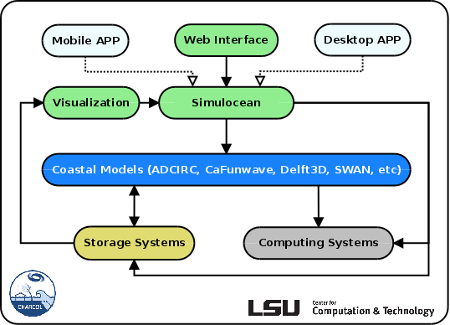
\includegraphics{../doc/_static/teakwood_flowchart.png}\hfill}


\chapter{Preview}
\label{preview:preview}\label{preview::doc}
1,This is the \href{http://localhost:8000/}{Teakwood}  welcome page. It provide you general information about teakwood, also it provide you a quick start tutorial, if you want to run jobs, sign in from the right top login entry. see:

\includegraphics{../doc/_static/teakwood_welcome.png}

2,After you signed in, you can start with models teakwood run.

{\hfill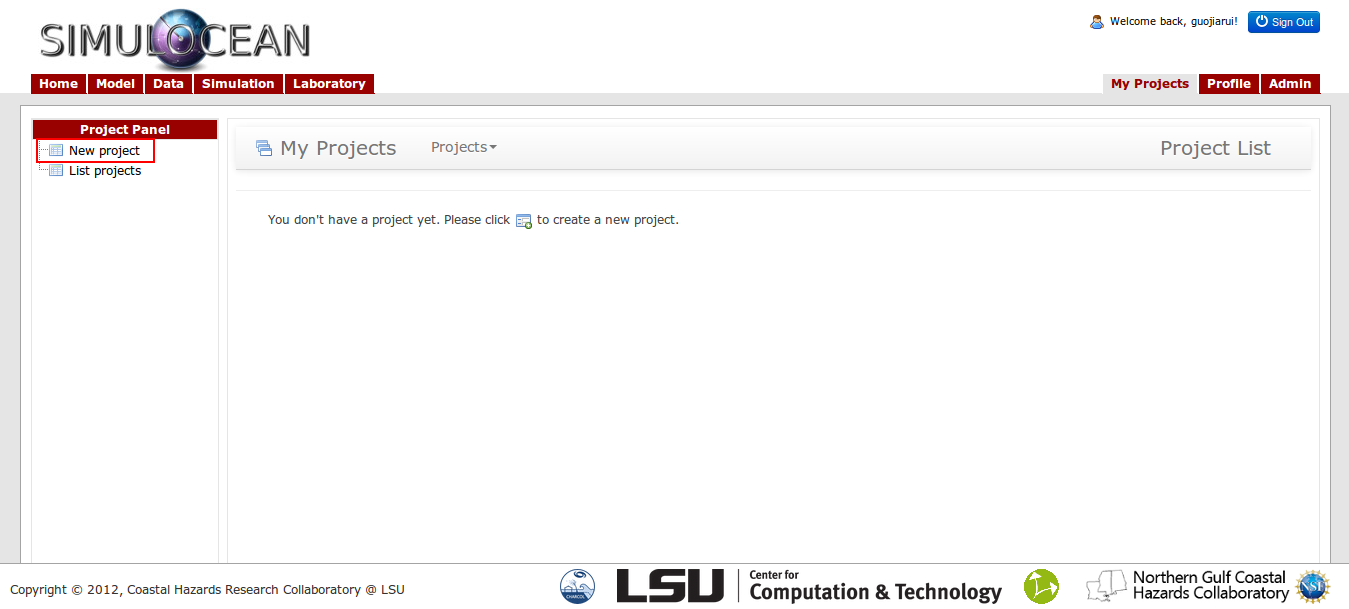
\includegraphics{workflow_projectmanagement.png}\hfill}


\chapter{Models}
\label{models:models}\label{models:teakwood}\label{models::doc}\setbox0\vbox{
\begin{minipage}{0.95\linewidth}
\textbf{Models}

\medskip


Currently Teakwood support five models: CaFunWAVE, Delft3D, SWAN, ADCIRC and FVCOM.
\end{minipage}}
\begin{center}\setlength{\fboxsep}{5pt}\shadowbox{\box0}\end{center}


\section{Delft3D}
\label{models:delft3d}
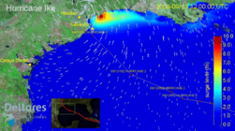
\includegraphics{models_delft3d.png}

Delft3D, developed by Deltares(formerly Delft Hydraulics), is a flexible integrated modelling suite, which simulates
two-dimensional (in either the horizontal or a vertical plane) and three-dimensional flow, sediment transport and
morphology, waves, water quality and ecology and is capable of handling the interactions between these processes.
After Delft3D-FLOW was open-sourced in 2011, more and more researchers started using Delft3D.


\section{CaFunWAVE}
\label{models:cafunwave}
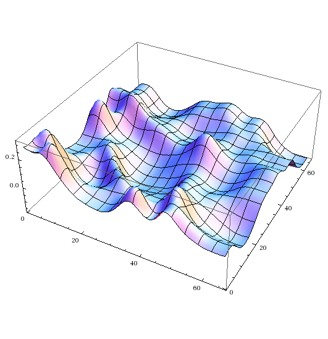
\includegraphics{models_cafunwave.jpg}

CaFunwave is a port of the Funwave-TVD code developed by Dr. Fengyan Shi and his colleagues at the University of
Delaware to the Cactus framework. By porting Funwave-TVD to the Cactus framework, we open the door to the possibility
of using new tools, such as Adaptive Mesh Refinement (AMR), different time stepping schemes, and the Chemora GPU
acceleration framework. A secondary advantage of the Cactus port is the ability to cross-check the codes against
each other to improve correctness and accuracy. CaFunwave is capable of simulating storm surges, tsunamis,
coastal nonlinear waves, wave-vegetation interaction, and breaking-generated near shore circulation.


\section{SWAN}
\label{models:swan}
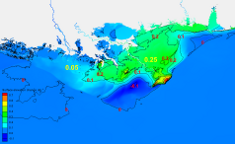
\includegraphics{models_swan.png}

SWAN is a third-generation wave model that computes random, short-crested wind-generated waves in coastal regions and
inland waters. SWAN accounts for the following physics: Wave propagation in time and space, shoaling, refraction due to
current and depth, frequency shifting due to currents and non-stationary depth, Wave generation by wind,
Three- and four-wave interactions, Whitecapping, bottom friction and depth-induced breaking, Dissipation due to vegetation,
Wave-induced set-up, Propagation from laboratory up to global scales, Transmission through and reflection
(specular and diffuse) against obstacles, and Diffraction.


\section{ADCIRC}
\label{models:adcirc}
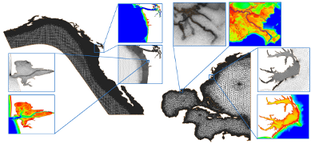
\includegraphics{models_adcirc.png}

ADCIRC is a system of computer programs for solving time dependent, free surface circulation and transport problems in
two and three dimensions. These programs utilize the finite element method in space allowing the use of highly flexible,
unstructured grids. Typical ADCIRC applications have included: (i) modeling tides and wind driven circulation,
(ii) analysis of hurricane storm surge and flooding, (iii) dredging feasibility and material disposal studies,
(iv) larval transport studies, (v) near shore marine operations.


\section{FVCOM}
\label{models:fvcom}
FVCOM is a prognostic, unstructured-grid, finite-volume, free-surface, 3-D primitive equation coastal ocean circulation
model developed by UMASSD-WHOI joint efforts. The model consists of momentum, continuity, temperature, salinity and
density equations and is closed physically and mathematically using turbulence closure sub-models. The horizontal grid is
comprised of unstructured triangular cells and the irregular bottom is presented using generalized terrain-following coordinates.
\setbox0\vbox{
\begin{minipage}{0.95\linewidth}
\textbf{Servers}

\medskip


Currently Teakwood provides conditional computing resources to our customers. more information about customer
levels please navigate to \href{http://localhost:8000/about/services/}{here}.
\end{minipage}}
\begin{center}\setlength{\fboxsep}{5pt}\shadowbox{\box0}\end{center}


\chapter{Submit a job step by step}
\label{demo:submit-a-job-step-by-step}\label{demo::doc}\label{demo:here}

\section{teakwood workflow}
\label{demo:teakwood-workflow}
{\hfill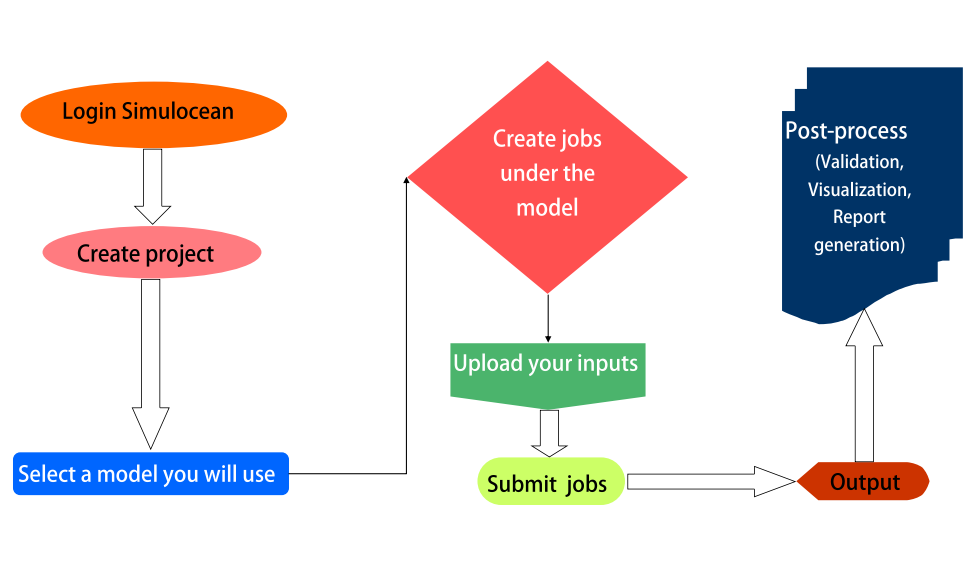
\includegraphics{jobworkflow.png}\hfill}

Teakwood provides multiple ways to help our user to use teakwood.

1) Magical wand.
Each page on the top right, there is a magical wand; it provides you detailed info of this page.


\includegraphics{magicalwand.png}

2) Video tutorial.
Please navigate to this \href{http://localhost:8000/about/contact/}{page} to see the video tutorial.

3) Step by step screen shots tutorial.
This page will give you a screen shot tutorial.

4)Post topic on teakwood forum if you have questions or encountered problems.
Please navigate to this \href{http://localhost:8000/about/contact/}{web page} to visit our forum.


\section{Handle your job in seven steps}
\label{demo:handle-your-job-in-seven-steps}
Since the workflow provided us a big picture of how Teakwood works, here are seven steps that can help us run
a general teakwood job.


\subsection{Create a \textbf{project}}
\label{demo:create-a-project}
In the first step, you will need to creating a project, Teakwood will generate an file management directory for you automatically.

{\hfill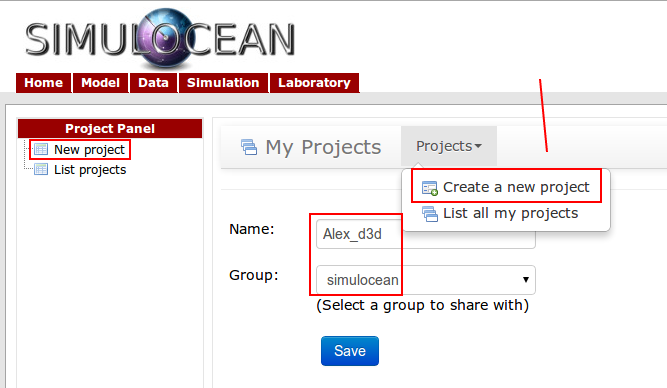
\includegraphics{cproject1.png}\hfill}


\subsection{Select a \textbf{model}}
\label{demo:select-a-model}
After project creating, you need to chose a model(e.g. Delft3D) for job running. We provide five models so far.

{\hfill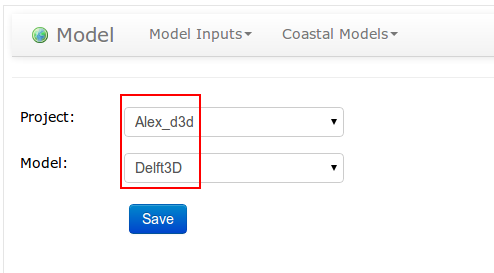
\includegraphics{cmodel1.png}\hfill}

{\hfill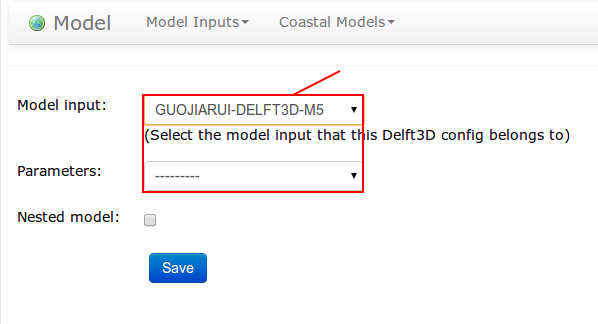
\includegraphics{cmodel2.png}\hfill}


\subsection{Create a \textbf{job}}
\label{demo:create-a-job}
You can create jobs underneath then.

{\hfill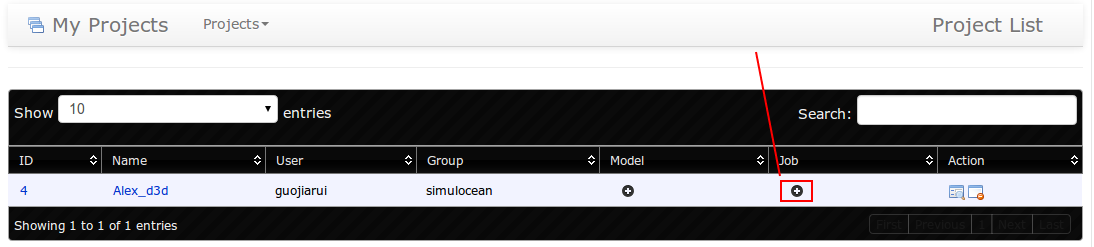
\includegraphics{cjob1.png}\hfill}


\subsection{\textbf{Insert} your input parameters}
\label{demo:insert-your-input-parameters}\begin{quote}

You can submit your input parameters either by \textbf{upload input files} or \textbf{fill in input forms}:
\end{quote}

{\hfill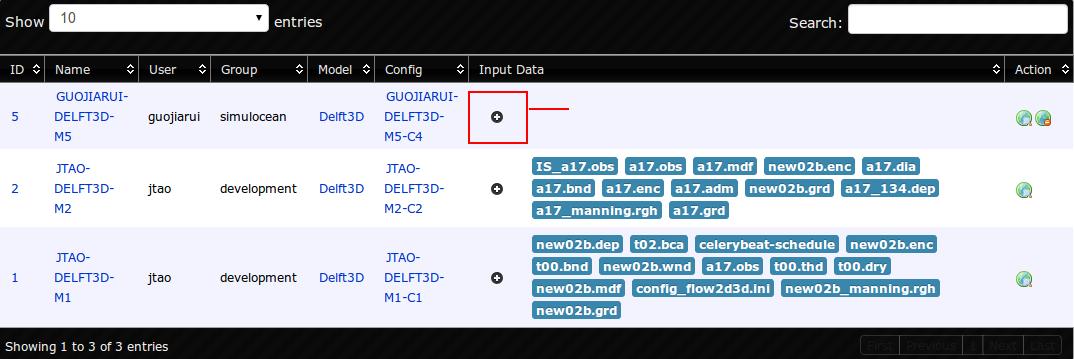
\includegraphics{cinput1.png}\hfill}

{\hfill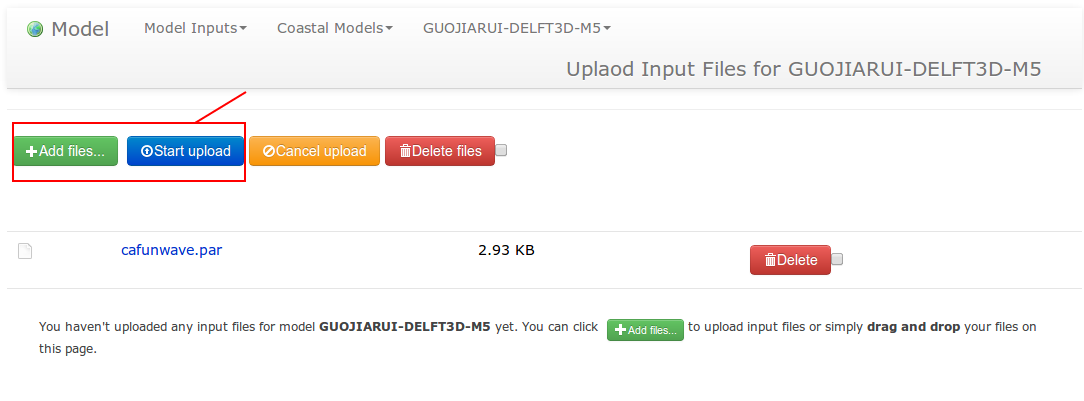
\includegraphics{cinput2.png}\hfill}


\subsection{\textbf{Submit} your job}
\label{demo:submit-your-job}
Simply submit your job, and your job will be in the waiting list and ready to go.


\subsection{\textbf{Check} status}
\label{demo:check-status}
Check status during the Job running from Teakwood control panel. All your jobs are under control.


\subsection{\textbf{Post-process}}
\label{demo:post-process}
In this step, we provide output data visualization and comparison. Details please see
\textbf{Chapter 5. Data Observation} segment in the directory.


\chapter{Coastal Data Factory}
\label{observation:coastal-data-factory}\label{observation::doc}\label{observation:web-page}\setbox0\vbox{
\begin{minipage}{0.95\linewidth}
\textbf{CDF(Coastal Data Factory)}

\medskip


Coastal Data Factory(CDF) is a toolkit for grabbing, storing, and visualizing coastal
data in the northern gulf and beyond. CDF provides an on-demand data grabbing engine, which allows users to easily
fetch data from both external data sources(e.g.NOAA, USGS) and internal CDF data center, and generates formatted data
for future use. The CDF client could be easily adapted as an independent tool for grabbing coastal
data. In our Teakwood framework, we use CDF to verify and validate simulation output.
\end{minipage}}
\begin{center}\setlength{\fboxsep}{5pt}\shadowbox{\box0}\end{center}

Coastal data factory(CDF) provides the following functions:


\section{Grabbing observational data.}
\label{observation:grabbing-observational-data}
Teakwood provides an on-demand data grabbing engine, so that user can easily fetch time series data from public data
sources(e.g.NOAA USGS).


\section{Host your data.}
\label{observation:host-your-data}
We provide free cloud storage to store your simulation data and crabbed data in standard formats.


\section{visualize your data.}
\label{observation:visualize-your-data}
CDF can transform your numerical data into dynamic charts so as to provide you an visual way of understanding your data.


\section{validate your computing result.}
\label{observation:validate-your-computing-result}
Though CDF platform,you can validate your computing result among your 1)standard referring data,
2)public observational data and 3) your simulation data.


\chapter{Report generation}
\label{report:report-generation}\label{report::doc}
Teakwood record each step of your job and generate an standard report afterward.
Hopefully this report will give you both big picture and details of your job and can be good reference towards paper
writing and presentation demo.

(we are still working on this model, and it will ready soon!)


\chapter{Host Teakwood in your machine}
\label{installation:host-teakwood-in-your-machine}\label{installation::doc}
After Installed Teakwood in your machine, you can
\begin{enumerate}
\item {} 
Deploy your own models in Teakwood.

\item {} 
Use your own Computing sources.

\end{enumerate}

This part will coming soon.


\chapter{Future Work}
\label{futurework:future-work}\label{futurework::doc}

\section{Scientific models}
\label{futurework:scientific-models}
We will deploy more and more scientific models in Teakwood.


\section{Visualization}
\label{futurework:visualization}
We will build in more and more visualization tool in Teakwood to help our users unveiling the abstract numerical output data.


\section{Submit your job to the world}
\label{futurework:submit-your-job-to-the-world}
Once provide credentials to Teakwood, Teakwood can submit your job to wherever machines you want, including commercial cloud.


\section{Data mining and Machine Learning}
\label{futurework:data-mining-and-machine-learning}
DM Provides a formal way of analysing output data and observational data;
ML provides a statistical way of predicting data, which is beyond classical physical function models.


\chapter{Version History}
\label{history:version-history}\label{history::doc}

\section{V0.90}
\label{history:v0-90}
V0.90 is the first version released.


\section{V0.91}
\label{history:v0-91}
Fixed some internal error links.
CafunWAVE model added.


\section{V0.92}
\label{history:v0-92}
FVCOM model added.


\section{V0.93}
\label{history:v0-93}
Plot model is ready.


\section{V1.0}
\label{history:v1-0}
Reorganized the structure of Teakwood Documentation.

© Copyright 2014, The Teakwood framework is distributed under the GNU Lesser General Public License (LGPL) v 3.0. This website
makes use of the wonderful icon sets by Studio MX and FAMFAMFAM. The icons used are distributed following the original
license respectively. Created using Sphinx 1.1.3.



\renewcommand{\indexname}{Index}
\printindex
\end{document}
